\section{Introduction}
In this chapter I will discuss the design aspect of the project, this will include an overview of the
architecture that I have decided upon and the rational behind it, I will then move to describe key components of
the design and how they relate to the aims and goals of this project and any interesting problems that they
may cause in the implemtation and how we propose to solve the problem. We will also briefly disscuss the
development plan that will be used to implement the system.

\section{Architectural Overview}
During the requirements analysis stage of this project it was clear that the project could be decomposed into
two main sub-modules, a front-end that will perform the interaction with the user and the operating system and a
back end that will process the user input in order to synthesis image this can be seen in 
Figure~\ref{fig:design_blocks}, the design of the project is such that the concerns of input and data processing
are seperated allowing for a cleaner design within each of the blocks. As we will be implementing the photon mapping
algorithm it is also clear that the back-end will contain two stages, the photon map generation which will produce the
photon maps that will in addition to the scene description from the front end be used to estimate the global illumination
of the scene.

\begin{figure}
\centering
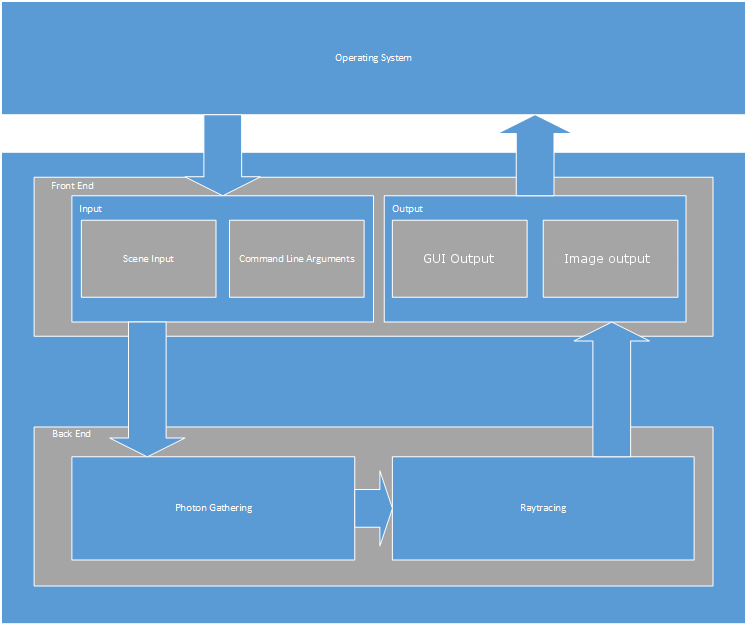
\includegraphics[scale=0.75]{./design/TopLevel.png}
\caption{Top level block diagram of the system}
\label{fig:design_blocks}
\end{figure}

\newpage
\section{Front End}
The front end of the system deals with the input and output of the system, this will manipulate and process
the input into a form that can be used by the backend to perform the synthesis, seperating the front and backend
allows the i/o and the synthesis to be modified with no modification required for the other block,
for intance the output could be an BMP image or a surface within a gui, the details of the conversion are
irrelevent to the back-end, only that the data passed to it is in a format that is understood.

\subsection{Scene Input}
The scene input takes in a description of a scene that is to be rendered from a file, this scene description
will give a listing of each of the objects in the scene such as meshes, lights and camera. Each of these
objects are also described by a file that is listed in the scene file. Each of the scene files are text files
that are human readable, this allows the files to be easily modified. Each of these configuration files allows
for attributes to be reused such as a material describing a mirrored surface can be defined in a single material
file that can be referenced by multiple objects. below is a list of the different scene files that are defined
(details of each of the files can be found in the appendix).

\begin{description}
\item[.scene] Top level description of the scene
\item[.mesh] Description of a mesh, including material and surface data.
\item[.mat] Description of a objects surface properties.
\item[.camera] Description of the camera in the scene.
\end{description}

\subsection{PLY mesh format}
One aspect of the mesh input file is a filename that referes to a PLY polygon mesh, it was decided that using
a pre-existing file format for the input to system was benificial as it allowed for assets from 3D modeling
utilities to be used to create the test scenes as they contain the required functionallity to export to PLY
meshes. the choice of the PLY made because it is a human-readable format (a binary PLY format is available but
not supported by the system) so as to fulfill requirement \todo{Add the requirement} that is also commonly used,
using PLY also allowed for example meshed from the Stanford PLY reposotory which in turn provided a selection of
relitivly complex models that could be used during the production and testing.

\begin{figure}
\lstinputlisting[language=C]{../Code/data/scenes/cornell_box.scene}
\label{fig:scene_file_example}
\caption{Example Scene File}
\end{figure}

\subsection{Command Line Arguments}
The program that is created must be able to take in more than one scene file to be useful, by having command
line arguments this allows the scene file to be changed without recompiling the code, there are other options
that are available including the number of threads that will be used to perform the raytracing and the
resolution and name of the output file, this will allow for the system to be used in scripts etc. refer to
Appendix\todo{Add the appendix} for full details of the command line options that are available.

\subsection{Image Output}
The image and gui block contains the code that will take the final pixel colours and presecnt them to the screen
there will be two modes of operation, image output and GUI output. Image output will store the output image
on the filesystem as a BMP file this allows the images to be saved.

\subsection{GUI}
In order to provide immediate feedback to the user it is nessaccarry to include a GUI in the system, this will
be a simple window that will display the progress of the system as it creates the images, this is usefull
for testing changes to a scene as it may be possible to see if the change has had the desired effect without
finishing what may be a costly render.

\subsection{Console Output}
In certain environments it is not possible to support a GUI (headless server) as a result the system includes
output on the console that inform the user of the progess of the render. \todo{expand}

\newpage
\section{Back End}
The back-end contains the code that deals with processing scene data, this block is decomposed into
two main blocks, the photon mapping block and the raytracing block, the photon mapping block is responsible
for the preprocessing step that creates the photon maps used to estimate the radiance. The raytracing stage
is responsible for computing the colour of each of the pixels in the output image, this will use the data
that was read into from the front end and the photon maps that were created by the photon map module. The
output of the raytracing block is sent to the front end which will use the data to present or save the final
image.

\subsection{Photon Emmition and Photon Map Construction (1 page)}
This block contains two stages, the photon emmition stage which traces photons through the scene and stores
the point of absorbtion and the balancing stage which sorts the photons into a data structure (left balanced
tree) that facilitated efficient storage and searching. The reason for the balancing stage is that the
distriburtion of the photons in the map is unlikely to be optimal \todo{Cite jensen book} and as this is a
preprocessing step it is worth the time to perform the balancing to improve later stages.

The construction of the photon map can be computationally expensive when a high number of photons are
requested to be created, in order to improve the performance of this stage multiple threads are created
that are responsible for emmitting a certain number of photons in the map, the number of threads will be
set in the front end and is configurable by the user to suit the machine that the system is being run on.

Each of the threads will trace photons through the scene as described in Algorithm\todo{Emmition Algorithm Ref}
once a photon has been found that will be stored in the photon map it will be written to a queue that is shared
by each of the threads, the photons have their power scaled as they are read from the queue.

The next stage in the pipeline reads photons from the queue, this will continue until each of the threads
has signalled that they have completed processing the photons, once all of the threads have been completed the
the list of photons will be transftered into the photon maps, this is the balancing stage.

\begin{figure}
\centering
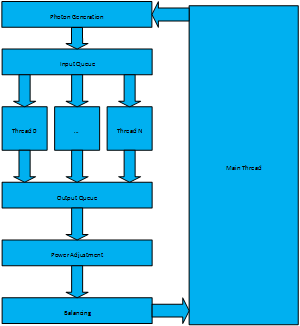
\includegraphics{./images/photon_threading.png}
\caption{Photon map generation}
\label{fig:photon_generation}
\end{figure}

\subsubsection{Multiple Photon Maps}
During the construction of the photon maps a choice must be made as to which of the photon maps the photon
should be placed in, this requires additional information to be passed from the emmition thread, this information
will describe the path that the photon has taken, this will in essence be an implementation of the path notation
that is commonly used to describe the path of a photon, in this case all paths will be stored in the global photon
map (\textbf{L(S\textbar D)$^+$D} in the path notation),only specular paths are stored in the caustic photon map
as these are the paths that contribute the most to the focusing effect of caustics (\textbf{LS$^+$D})


\subsection{Raytracing (1 pages)}
As can be seen from Figure~\ref{fig:design_blocks} the raytracing module contains $n$ threads, each of these
threads trace a subset of the pixels in the image and run independantly to each other, this is possible due
to the inherent parrellism in the photon mapping algorithm. This stage in the system will perform raytracing
as described in \todo{cite}, for each intersection found during the running of the system the photon
maps created during previous stage will be used to estimate the radiance of the point in order to estimte the
true illumination at the point factoring in the global effects.

\begin{figure}
\centering
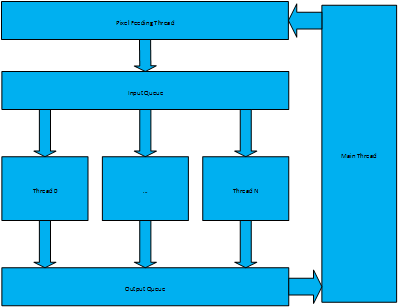
\includegraphics{./images/pixel_threading.png}
\caption{Raytracing architecture}
\label{fig:pixel_generation}
\end{figure}

The architecture of the raytracing block shared many simalarities with that of the photon emittion stage,
it is also a pipeline, there is a threads that inputs each pixel in the output image to a queue, this queue
is in turn read by one of multiple threads that perform photon mapping for a ray emmited through the pixel,
multiple rays are generated for each pixel performing distrubution raytracing, the colour of the pixel is
then written to an output queue that will be read by the main thread in order to send the pixel values to
the front end to be presented to the user.

\subsubsection{Distribution Raytracing}
Each of the raytracing threads performs distribution raytracing, this is a commonly used adjustment to the 
raytracing algorithm that allows for simulation of fuzzy phenomena such as soft shadows and glossy reflection
models, as described by Jensen \todo{cite} distribution raytracing can also be used to estimate the contribuiton
of diffuse intereflection, at each intersection of the eye ray a diffuse refeltive \todo{this is only true of
diffuse surfaces} ray is generated, this ray is then traced into the scene, at the intersection point of this ray
we use the photon map to estimate the radiance leaving the surface in the direction of the original intersection
point, as we are tracing multiple rays per pixel an estimate of the global illumination is found by averaging each
of these reflective rays.

\begin{figure}
\missingfigure{Algorithm For distributiuon raytracing}
\end{figure}

\subsection{Objects}
Much of the raytracing algorithm that is performed on each of the
objects in a scene are the same, for example finding a refracted
ray is only dependant on the surface noraml at a point of intersection
for this reason the system abstracts any object that can be intersected
must implement certain functions, this is a form of object orentation.
e
\subsection{Materials}
\subsection{Participating Media}


